\documentclass[border=10pt]{standalone}
\usepackage{pgfplots}
\pgfplotsset{compat=1.18}
\begin{document}
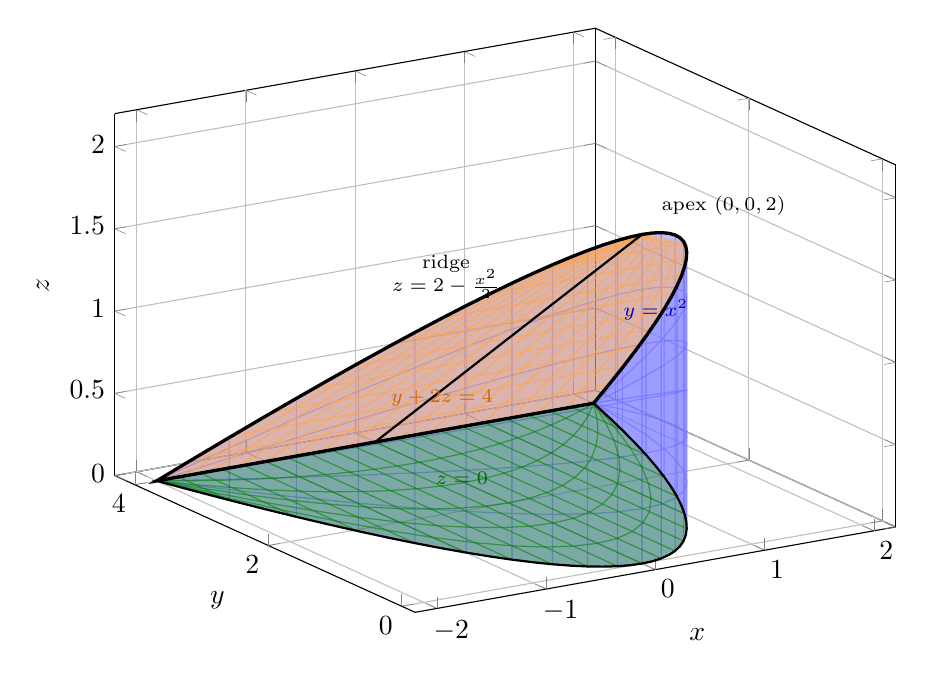
\begin{tikzpicture}
\begin{axis}[width=11.5cm, height=9cm, view={-32}{24},
    xlabel={$x$}, ylabel={$y$}, zlabel={$z$},
    xmin=-2.2,xmax=2.2, ymin=-0.2,ymax=4.3, zmin=0,zmax=2.2, grid=major]
  \addplot3[surf, shader=flat, domain=-2:2, y domain=0:1, samples=21, samples y=7,
            blue!55, opacity=0.45] ({x},{x*x},{y*(2-x*x/2)});
  \addplot3[surf, shader=flat, domain=0:2, y domain=-1:1, samples=11, samples y=17,
            orange!70, opacity=0.45] ({y*sqrt(4-2*x)},{4-2*x},{x});
  \addplot3[surf, shader=flat, domain=-2:2, y domain=0:1, samples=21, samples y=7,
            green!50!black, opacity=0.35] ({x},{x*x+y*(4-x*x)},{0});
  \addplot3[very thick, domain=-2:2, samples=41] ({x},{x*x},{2-x*x/2});
  \addplot3[thick, domain=-2:2, samples=41] ({x},{x*x},{0});
  \addplot3[thick, domain=-2:2, samples=41] ({x},{4},{0});
  \addplot3[dashed, thick, domain=0:2, samples=11] ({0},{4-2*x},{x});
  \node[font=\scriptsize, anchor=south west, text=black] at (axis cs:0.15,0.1,2.02) {apex $(0,0,2)$};
  \node[font=\scriptsize, text=blue!80!black] at (axis cs:1.5,2.25,0.95) {$y=x^2$};
  \node[font=\scriptsize, text=orange!80!black] at (axis cs:0,3.0,0.45) {$y+2z=4$};
  \node[font=\scriptsize, text=green!40!black] at (axis cs:0,2.7,0.02) {$z=0$};
  \node[font=\scriptsize, text=black, align=center] at (axis cs:-1.55,0.4,1.85) {ridge\\[-2pt] $z=2-\frac{x^2}{2}$};
\end{axis}
\end{tikzpicture}
\end{document}
